\documentclass[12pt]{article}

\title{Semantics of Fake News Detection using BERT}
\author{Carmen Thom}
\date{04.03.2024}

\usepackage[margin=1in]{geometry}
\usepackage{times}
\usepackage[table,xcdraw]{xcolor}
\usepackage{graphicx}
\graphicspath{ {./img/} }
\usepackage{caption}
\usepackage{setspace}
\usepackage[backend=biber,style=ieee,sorting=ynt]{biblatex}
\addbibresource{references.bib}
\begin{document}
\maketitle
\onehalfspace


In the information era, where the breadth of human knowledge is available at a moments notice, the human race has never before seen potentials. However, through the means of bad actors and misinformation, fake news is also more prominent than ever. "websites hosting AI-created false articles have increased by more than 1,000 percent, ballooning from 49 sites to more than 600, " \cite{Verma_2023}. At the same time as this information is growing, the scope, class, and detectability of AI is growing rapidly. However, AI can also be used for good. With fake news spreading as rapidly as it is, being able to classify fake news accurately becomes out of our scope. Using a contextual transformer models that excels at language in context, BERT, I built a binary classifier to analyze the semantics of errors and what that may say about fake news. Similar research has been done using Latent Semantic Analysis as a mean to classify fake news, however modern NLP tools excel strongly with the use of transformer models, outperforming the neural network architecture used in LSA. \\

In the world of semantic and pragmatic language analysis, fake news can be thought of as a news source with beliefs incompatible with our current systems of understanding. Fake news detection is hard for both humans and machines. Even with valid arguments, you still can reach false conclusions. Soundness is much harder for people to detect, which makes the task more nuanced. There is also framing that makes fake news detection hard, as two events can be framed very differently using words with similar meanings but differing senses. BERT can handle homographs such as "bank" the financial institution and "bank" of a river, assigning them to different vectors in a vector space. On a generalized scale, BERT masks words in a sentence, and is trained on prediction of word to create those contextual embedding of a vector space. The sentence "I like semantics" would be tokenized to [[CLS], "I", "like", "semantics", [SEP]], which could be masked to [[CLS], "I", [MASK], "semantics", [SEP]], in which a probability space would be sampled, giving a distribution of likelihoods of tokens for the mask token. This makes the task of training a BERT model technically a supervised task, while being fed an unsupervised dataset. \\

For this project, the dataset used was WELFake dataset \cite{9395133}. To diversify the sources, the original authors compiled sources from Kaggle, McIntire, Reuters, BuzzFeed Political. The dataset contains 72,134 news articles, 35,028 with label 1 for real, and 37,106 with label 0 for fake. The class proportions don't seem to have a statistically significant skew, meaning that the data appears well balanced. For fine tuning on this dataset, I went with 0.7 partitioned for training, with the .3 remaining being split between validation and testing. \\

BERT models, as they use transformer architecture, excel at transfer learning. Thus, fine-tuning a pretrained BERT model was the best way to develop the classifier. For the pretrained model, I used Google's \verb|bert_uncased_L-4_H-512_A-8| model. This is significantly computationally easier to pretrain than the most used \verb|bert-base-uncased| model as the hidden size is reduced by a third, as well as fewer layers and attention heads. This change also reduced the odds of the fine-tuned binary classification model being over-fit. With larger datasets, further computational resources, as while as more dedicated training time, the model size could be increased. For this reason, the model is left as a hyperparameter in the \verb|main| function of \verb|model.py|. Relevant hyperparameters were all placed at the beginning so it could be easily manipulated by other researchers.\\

For fine-tuning, I used the transformers \verb|BertForSequenceClassification| built on PyTorch's neural network modules. A batch size of 64 was used to have less computational processes, although a lower batch size may have been ideal to help model generalization, and would keep keeps less data in local memory which is useful. I ran the model with 5 epochs. 3 may have been sufficient as the dataset is middle-sized, but checkpointing on training epochs was not implemented in the first run through so stopping when the model began to have marginal decreases in loss was not an option. \cite{devlin2019bert} Checkpointing has now been implemented, but on a 8 core system, fine-tuning took approximately 4 hours. This could be greatly improved with access to a GPU, and with access to a Google Cloud TPU training should run well under an hour. For loss criterion, many of the academic and industrial papers fine-tuning BERT for binary sequence classification use a cross-entropy loss function which was also the criterion I chose. \\

Running the final evaluation script, the model obtained a macro average F1-score of 0.98, suggesting the model is performing extremely well. Looking at the confusion matrix, we nearly see a diagonal matrix, supporting the belief in model excellence. Testing could be diversified with news external to this dataset to test generalization. In further iterations, it would also be beneficial to analyze the classification as a continuous variable in the domain of [0,1] to implement some form of weighting to the evaluation based on model confidence. \\
\begin{center}
\textbf{Performance Metrics and Confusion Matrix}
\end{center}
\begin{figure}[h]
  \centering
  % First image
  \begin{minipage}{0.48\textwidth}
    \centering
    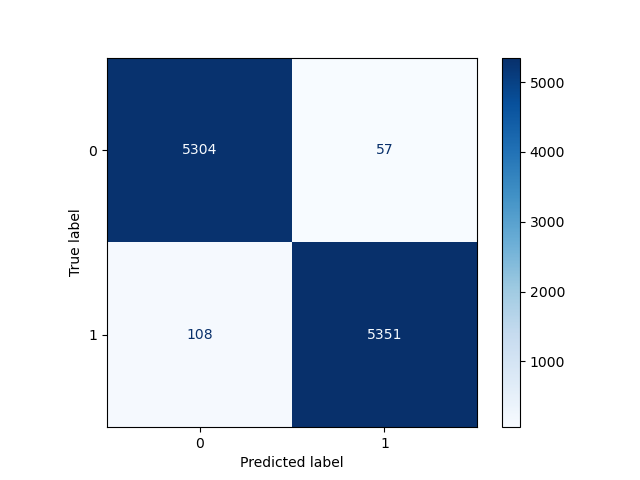
\includegraphics[width=\linewidth]{confusion}
    \caption{Confusion Matrix}
  \end{minipage}
  \hfill
  % Second image
  \begin{minipage}{0.48\textwidth}
    \centering
    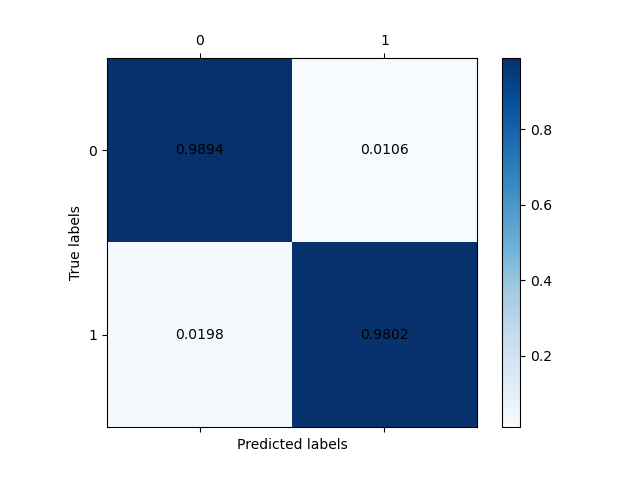
\includegraphics[width=\linewidth]{norm_confusion}
    \caption{Normalized Confusion Matrix\\~\\}
  \end{minipage}
\end{figure}
\begin{minipage}{\textwidth}
\centering
\begin{tabular}{|
>{\columncolor[HTML]{F5F9FE}}l |l|l|l|l|}
\hline
\cellcolor[HTML]{08306B} & \multicolumn{1}{c|}{\cellcolor[HTML]{F5F9FE}Recall} & \multicolumn{1}{c|}{\cellcolor[HTML]{F5F9FE}Precision} & \multicolumn{1}{c|}{\cellcolor[HTML]{F5F9FE}F1-Score} & \multicolumn{1}{c|}{\cellcolor[HTML]{F5F9FE}Support} \\ \hline
0                        & 0.98                                                & 0.99                                                   & 0.98                                                  & 5361                                                 \\ \hline
1                        & 0.99                                                & 0.98                                                   & 0.98                                                  & 5459                                                 \\ \hline
Accuracy                 &                                                     &                                                        & 0.98                                                  & 10820                                                \\ \hline
Macro Average            & 0.98                                                & 0.98                                                   & 0.98                                                  & 10820                                                \\ \hline
Weighted Average         & 0.98                                                & 0.98                                                   & 0.98                                                  & 10820                                                \\ \hline
\end{tabular}
\captionof{table}{Evaluation metrics}
\end{minipage}
\\~\\

On inspection of the Type-1 errors, false positives, I found that most were in the first person. using pronouns like "I" while describing events. This could be attributed to personal reporting and accounts perhaps being more likely to be lies, which leads the model to attributing person to fake news. The type 2 errors seemed to be accounts from politicians and other elected officials. My current belief for why this may be is that generally accounts from officials should be classified as truth, so the model is less likely to accurately identify their misinformation.\\

To conclude, the type-1 and type-2 errors of this model reveal semantic information of what gets past detection software. While these models perform better than LSA models, the predecessor still has important uses in NLP, and provide an alternative interpretation of the classification. With the spread of misinformation on the internet, for sanctity of knowledge for future generations detection of fake news on the internet is important. While legislation could benefit this issue, especially in regard to spread of misinformation through AI, there is a slippery slope. With tools now available, I think it is in the best interest to use these tools as a mean to detect possible misinformation, for it to be further evaluated by human analysts. The modern spread of fake news needs modern solutions, and NLP models are that solution.
\pagebreak

\nocite{*}
\printbibliography
\end{document}